\documentclass[12pt,letterpaper,titlepage]{article}
\usepackage{solarized-light}
\usepackage{fontspec}
\defaultfontfeatures{Mapping=tex-text}
\usepackage{xunicode}
\usepackage{xltxtra}
\usepackage{amsmath}
\usepackage{pdfpages}
\usepackage{amsfonts}
\usepackage{bbold}
\usepackage{amssymb}
\setcounter{secnumdepth}{0}
\usepackage{nameref}
\usepackage{enumitem}
\usepackage{environ}
\usepackage{pgfplots}

\showboxdepth=\maxdimen
\showboxbreadth=\maxdimen


\usepackage{paracol}
\usepackage{wrapfig}
\globalcounter{table}
\globalcounter{figure}
\usepackage{graphicx}
\usepackage[left=1in,right=1in,top=1in,bottom=1in]{geometry}
\graphicspath{{img/}}

\author{Jacob Abel}
\title{	Project 2
	\\\large ECE2500 CRN:82943
}

\setlength{\parskip}{0.5em}

\begin{document}
\maketitle
\begin{raggedright}

\section{Summary}
This project involved the development of a MIPS Assembly function to compute the greatest common denominator of the inputs and the implementation of the required instructions in Verilog to run said function. The iterative C function that the Assembly is based on is included in Appendix A.

\section{Assembly Design}
The function was relatively simple to implement. Each standard form (if, for, while, do-while) in the C function was delimited by labels in the assembly source. At this point the labels were filled in with the corresponding assembly to each standard form. Minor mistakes were made such as writing a bne instead of a beq but these were easily resolved by analysing the failing loops. The function ended up requiring the following functions: beq, bne, andi, or, addi, srl, sll, slt, \& sub. These are implemented in the next section. The main function for the QTSpim simulation was a series of straightforward load immediates, moves, and jump-and-links. As such the design was trivial. The simulation results of the QTSpim run are in Appendices B and C. 

\section{Verilog Design}
The modifications to the existing Verilog were also fairly trivial. Within \texttt{mips-control.v} each instruction was added to the \texttt{casex} based on their corresponding values from the MIPS Reference Sheets. The procedural blocks for each statement was adopted from their corresponding instruction types. The R-types adopted from the sll instruction and the I-types were adopted from the addi instruction. The ALU codes were determined by reading \texttt{mips-alu.v}. Branching was implemented by adding a 2x1 mux and 2 dataflow statements to \texttt{mips.v}. The dataflow statements generated the branch PC address and the enable bit for the mux. The mux rerouted the input to the PC reg from the incrementer to the branch address when the enable bit was high. The branch instructions were adopted from the R-type's procedural block and the \texttt{branch\_out} wires were enabled. The \texttt{jump\_out} was re-purposed as an enable for inverting the branch's zero check. Luckily no debugging was required as the project compiled and simulated correctly on the first attempt. The simulation results are in Appendix D.

\clearpage
\section{Appendix A: GCD C Source}
\begin{center}
\lstinputlisting[language=C]{src/bGCDit.c}

Iterative C Greatest Common Denominator Function (courtesy Wikipedia)
\end{center}

\clearpage
\section{Appendix B: BinaryGCD in QTSpim prior to running}
\begin{center}
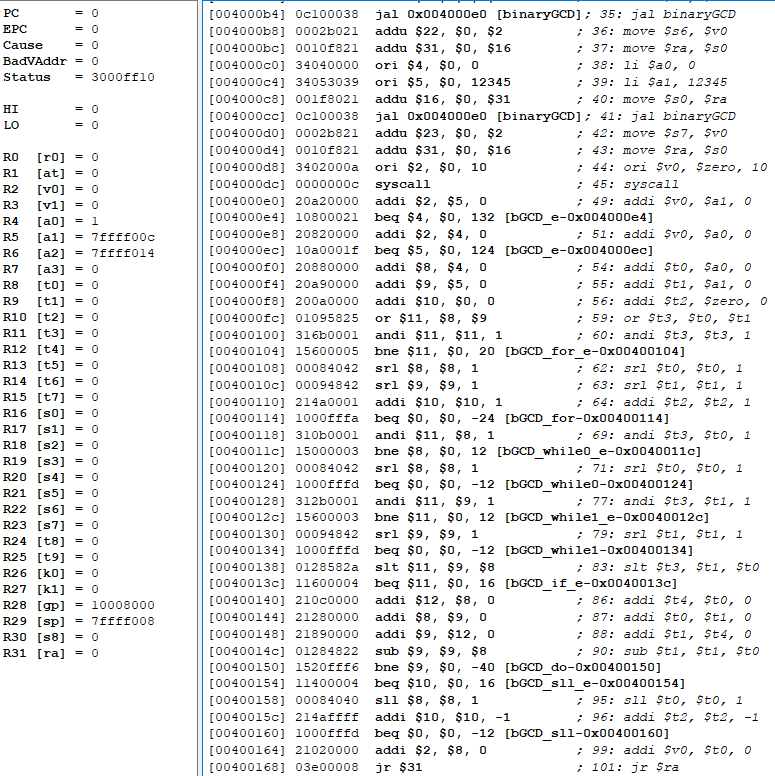
\includegraphics[width=\textwidth, height=\textheight, keepaspectratio=true]{pre}
\end{center}

\clearpage
\section{Appendix C: BinaryGCD in QTSpim after running}
\begin{center}
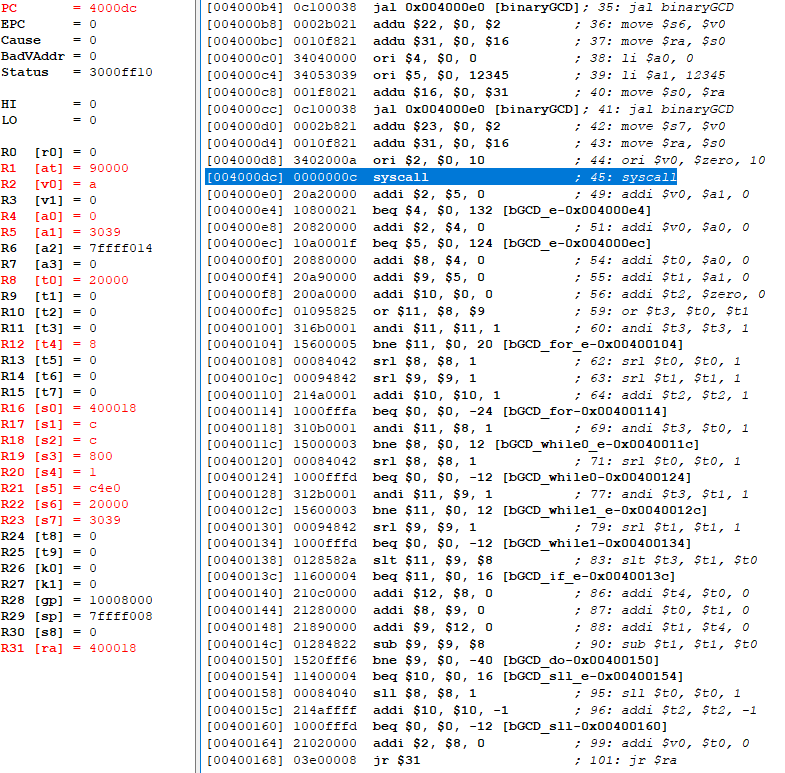
\includegraphics[width=\textwidth, height=\textheight, keepaspectratio=true]{post}
\end{center}

\clearpage
\section{Appendix D: Modelsim waveform of BinaryGCD(12, 780)}
\begin{center}

At Initialisation

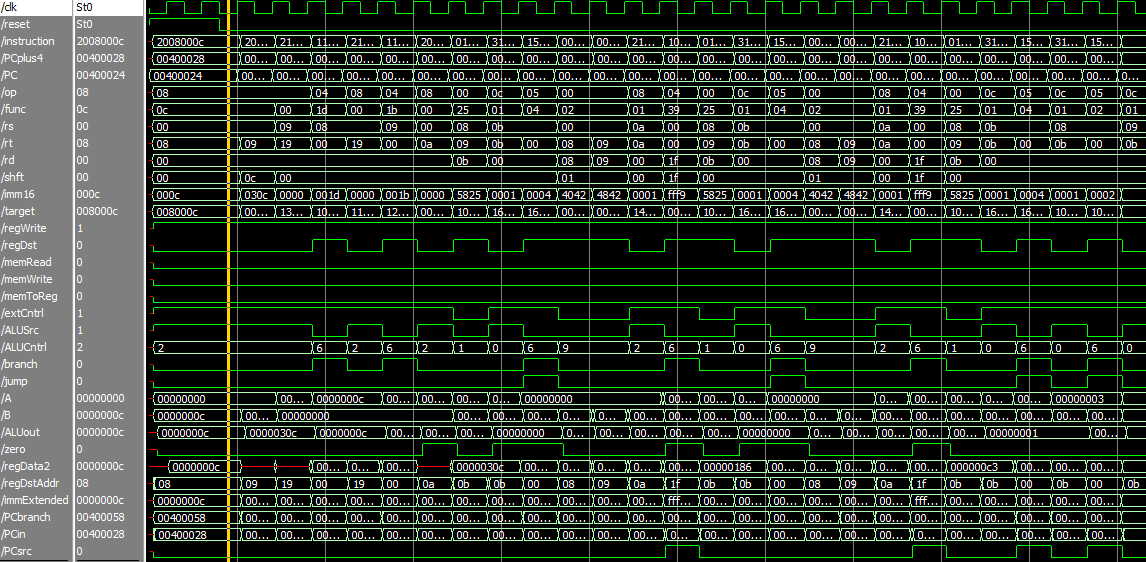
\includegraphics[width=\textwidth, height=\textheight, keepaspectratio=true]{wav_pre}

Full Run (Including Final Results)

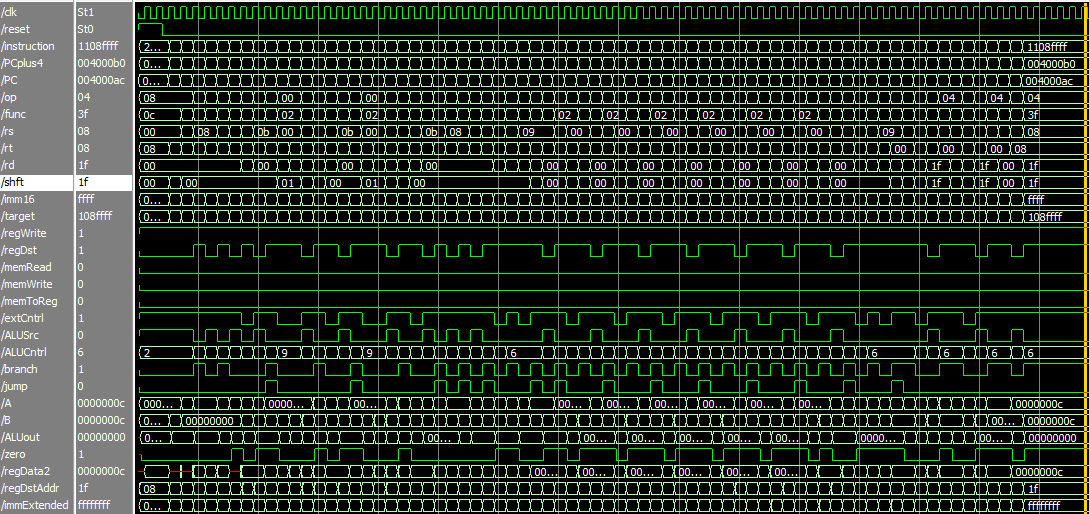
\includegraphics[width=\textwidth, height=\textheight, keepaspectratio=true]{wav_post}

\end{center}

\end{raggedright}
\end{document}